\section{Learning Outcomes}

By the end of week 2, you should be able to:

\begin{enumerate}
\item Still do everything described in the script for lab session 1.
\item Manipulate strings.
\item Use Boolean variables.
\item Use tuples and lists.
\item Use the {\tt input} command.
%\item use indentation and colons.
\end{enumerate}


\section{Preamble} 

Today you'll work through several sections that introduce various features of \texttt{Python}. Typically there will be one or more exercises at the end of each section; make sure you work on these before moving on. Ask for help if you're unsure or get stuck, its what we're here for!

% \subsection{Managing your time: Typical students}
% If this is your first experience with programming, then the following is a general guide as to how to manage your time during the lab sessions. You should easily be able to get 70\% in the three assessments, but you may well find that it is not a good use of your time to try to get up to 100\%. Rest assured that by the middle of year two, there will be no difference in skills between currently "rookie" programmers and those who have been coding since they were in primary school. 

% If you feel that you're falling behind, don't panic. Ask for help and use the "gap weeks" (see below) to catch up.

% The "gap weeks" fall in the weeks that assessments are due (4, 7, 10). Lab sessions in these weeks are optional, but you are strongly encouraged to make use of them, to:

% \begin{itemize} 
% \item Get verbal feedback on your assessments.
% \item To catch up with any exercises in the lab scripts that you have not finished yet. Note that model answers to the exercises will be put on Study Direct during the respective gap week.
% \item To take one of the three optional (but recommend) "competency" tests that feed into the end of term skills certificate.
% \item Do project work. 
% \end{itemize}

% \subsection{Managing your time: Advanced students}
% If you already feel comfortable with programming have and/or have ambitions to use programming for problem solving (including for the optional  project) and/or for career advancement, then you should aim to finish the whole problem sheet, including {\bf advanced exercises} by the week of the respective lab session (this will probably include work done in your own time between sessions). You are welcome to ask the ATs for feedback on your codes ({\it please only ask for help with advanced exercises during the gap weeks and after checking the model solutions)}. We suggest forming a study group with peers at a similar level: collaborative coding is efficient coding (but please develop your assessment solutions individually). The advanced exercises will help you prepare to score highly on the assessments.

% If you want to focus on project work towards the end of term, then by all means work through the session sheets at a faster rate than the rest of the class, and hand in your assessments early.

\subsection{A reminder about collusion and plagiarism}
\label{subsec:collusion}
Don't do it. By all means work together on the exercises during the lab sessions, and by all means {\it talk} to each other about ways to approach the assessments. However, if find yourself de-bugging a friend's code for an assessment, you've gone too far -  you've got to let them figure this stuff out themselves. If you find yourself cutting and pasting from a friend's code, then that's even more serious. If incidences of plagiarism and collusion do come to light, those involved will be referred to the appropriate disciplinary committee. 

\subsection{Sourcing Help}
When coding, in this module or in the future, you may run into inexplicable errors or wonder what the best approach to a problem is. By all means ask the ATs for help but you should also be aware of \url{www.stackoverflow.com}, a community driven forum where people post their problems and users attempt to provide solutions. If you run into a problem it's almost certain that somebody else has already had it, and asked about it somewhere on the internet, so it's worth having a look.
As an aside, if you get a large, confusing error message in a Jupyter notebook, you can look for a \texttt{->} symbol near the top, and that will show you the line of code that failed to execute.

\section{String manipulations}

\noindent Now on with today's session. In the previous chapter you were introduced to strings, a data type containing characters. Strings can be manipulated very easily with inbuilt operators (literally a symbol that performs an operation on a variable) such as \texttt{`+'}, which can be used to add strings together (concatenate them). Strings can be `indexed' to extract specific characters or sliced with the \texttt{`:'} operator to extract a set of multiple characters. \textbf{Note that \texttt{Python} starts counting elements from zero}, which means that the first character in a string is character zero. Here are some examples, try then all in your \texttt{jupyter} notebook.\\ 

We can add strings to concatenate them.
\begin{lstlisting}[style=PY] 
In [1]: # Define strings for manipulation
        s1 = "This is a"
        s2 = "string"
        
        print(s1 + ' ' + s2)
\end{lstlisting}
\begin{lstlisting}[style=PY_out]
        This is a string
\end{lstlisting}
We can index a specific element by indexing with square brackets (note: an element of a string includes characters and \textbf{also} whitespaces). This is also a good time to point out that the \texttt{print} can print as many variables as you like, just seperate them with a comma:
\begin{lstlisting}[style=PY] 
In [2]: # Print the first and last element of s1 to demonstrate indexing
        print(s1[0], s1[-1])
\end{lstlisting}
\begin{lstlisting}[style=PY_out]
        T a
\end{lstlisting}
Notice we can extract the final element by indexing with -1. In fact we can count back from the end of a string with n characters by using a negative index (i.e. -1 extracts the n$^{\text{th}}$ character \textbf{a}, -3 extracts the n-2$^{\text{th}}$ character \textbf{s}, -4 extracts the n-3$^{\text{th}}$ character \textbf{i}, etc.).\\

We can also slice with indices by using the \texttt{:} operator, [start index:end index]. Bear in mind that \texttt{Python} indexing is inclusive of the start index and exclusive of the end index, so [0:4] would only retrieve characters 0, 1, 2, and 3.
\begin{lstlisting}[style=PY]
In [3]: # Slice the string to get the first 6 elements
        print(s1[0:7])
\end{lstlisting}
\begin{lstlisting}[style=PY_out]
        This is
\end{lstlisting}
\begin{lstlisting}[style=PY]
In [4]: # Get the second to the 4th elements
        print(s1[1:4])
\end{lstlisting}
\begin{lstlisting}[style=PY_out]
        his
\end{lstlisting}

Additionally strings can be multiplied by integers to make them repeat. 
\begin{lstlisting}[style=PY]
In [5]: # Print 'This' three times separated by spaces
        print(s1[:5] * 3)
\end{lstlisting}
\begin{lstlisting}[style=PY_out]
        This This This 
\end{lstlisting}
Final thing to note with slicing is that the 0 (first index) can be omitted as in the previous example. \texttt{Python} sees this as `from the beginning', the same is true for the end if the second index is omitted (\texttt{[2:]}, i.e. the 3rd element to the end).

\subsection{Exercises}
\subsubsection{Exercises (with solutions at the end of the chapter)}
\label{Strings}

Try the following (for answers see Section~\ref{workedanswerslab2})
\begin{enumerate}
\item
\begin{enumerate}
\item Assign the strings `\texttt{hello}' and `\texttt{world}' to two separate variables.
\item Using the two strings print out `\texttt{hello world}'
\item Print the word hello 20 times with no spaces using the assigned string.
\end{enumerate}
\item
\begin{enumerate}
\item Declare a variable and assign the following string to it `\texttt{Do not push the red button}'
\item Slice the string to form `\texttt{Do not push}'
\item Slice the string to form `\texttt{push the red button}'
\end{enumerate}
\end{enumerate}

\subsubsection{Exercises (other)}

\begin{enumerate}
\item W2Basic1 - Create a string variable \texttt{myname} that is your full name - first, middle (if you have them) and last (family name).
\begin{enumerate}
      \item Slice the string so that it prints your last name only.
      \item Slice the string such that it prints your first name, middle initial and then your last name.
      \item Print `I am' and your name.
\end{enumerate}
\end{enumerate}

\section{Boolean Variables}
\label{boolvars}

\textbf{Boolean} expressions represent the two values of Boolean logic, \texttt{True} or \texttt{False}. They can be used to compare variables, if the variables are the same then the result will be \texttt{True}, and if they are not then the result will be \texttt{False}.

\textbf{Note:} If the variables are of a different type (float and integer), but are the same number, the result will be \texttt{True}, for instance \texttt{1 == 1.0} will return \texttt{True}. This is not true if one variable contains a string and another a float or integer, \texttt{`1' == 1} will return \texttt{False}.

\begin{lstlisting}[style=PY] 
In [1]: # Define variables to demonstrate Boolean operations
        a = 12
        b = 5
        c = 7.8
        
        # Test if a is equal to b
        a == b
\end{lstlisting}
\begin{lstlisting}[style=PY_out]
Out[1]: False
\end{lstlisting}
\begin{lstlisting}[style=PY]
In [2]: # Test if a is greater than or equal to c
        a >= c
\end{lstlisting}
\begin{lstlisting}[style=PY_out]
Out[2]: True
\end{lstlisting}
Multiple boolean expressions can be tested at once using the keyword \texttt{`and'}.
\begin{lstlisting}[style=PY]
In [3]: # Test if b is greater and c and b is greater than a
        print(b > c and b > a)
\end{lstlisting}
\begin{lstlisting}[style=PY_out]
        False
\end{lstlisting}
Multiple boolean expressions can also be combined without \texttt{`and'}
\begin{lstlisting}[style=PY]
In [4]: # Test whether a is greater than c and c is greater than b,
        # without using and
        print( b < c < a )
\end{lstlisting}
\begin{lstlisting}[style=PY_out]
        True
\end{lstlisting}

Table~\ref{BooTab} summarises the Boolean operators . [Note that you can also use {\tt in} but only with tuples and lists, see Table~\ref{StringTab}.]

\begin{table}[!h]
\begin{center}
\begin{tabular}{|l | p{4cm}|}
\hline
\texttt{==} & Equal to\\\hline
\texttt{!=} & Not Equal to\\\hline
\texttt{>=} & More than or equal to\\\hline
\texttt{<=} & Less than or equal to\\\hline
\texttt{>} & More than\\\hline
\texttt{<} & Less than\\\hline
\end{tabular}
\end{center}
\caption{Boolean operators available in \texttt{Python}. Note that you can also use \texttt{in} to check if something is in a list or tuple, it'll return a Boolean.}
\label{BooTab}
\end{table}

\newpage

\subsection{Exercises}

\begin{enumerate}
\item W2Basic2 - Assign 13 to a variable $q$, 2 to a variable $w$, and 6.5 to a variable $e$.
\begin{enumerate}
      \item Check that $q$ is less than $w$.
      \item Check that $q\div$2 is equal to $e$.
\end{enumerate}
\end{enumerate}
\noindent Note: for these exercises, make sure a {\tt True} or {\tt False} is displayed on screen as needed.\\

\section{Tuples \& Lists}
The following data types are commonly stored in lists or tuples:
\begin{itemize}
    \item Integers
    \item Floats
    \item Strings
    \item Boolean
\end{itemize}

\noindent In fact any \texttt{Python} object can be stored in a list or tuple. That includes other lists and tuples, so it is possible (and sometimes useful) to have a list of lists. As mentioned in section \ref{dtypes}, lists and tuples are essentially the same; the key difference is that lists are mutable (editable) and tuples are not. Figure \ref{fig:listtup} shows the general structure of these objects. 

\subsection*{Anatomy of Lists and Tuples}
\begin{figure}[H]  
\centering
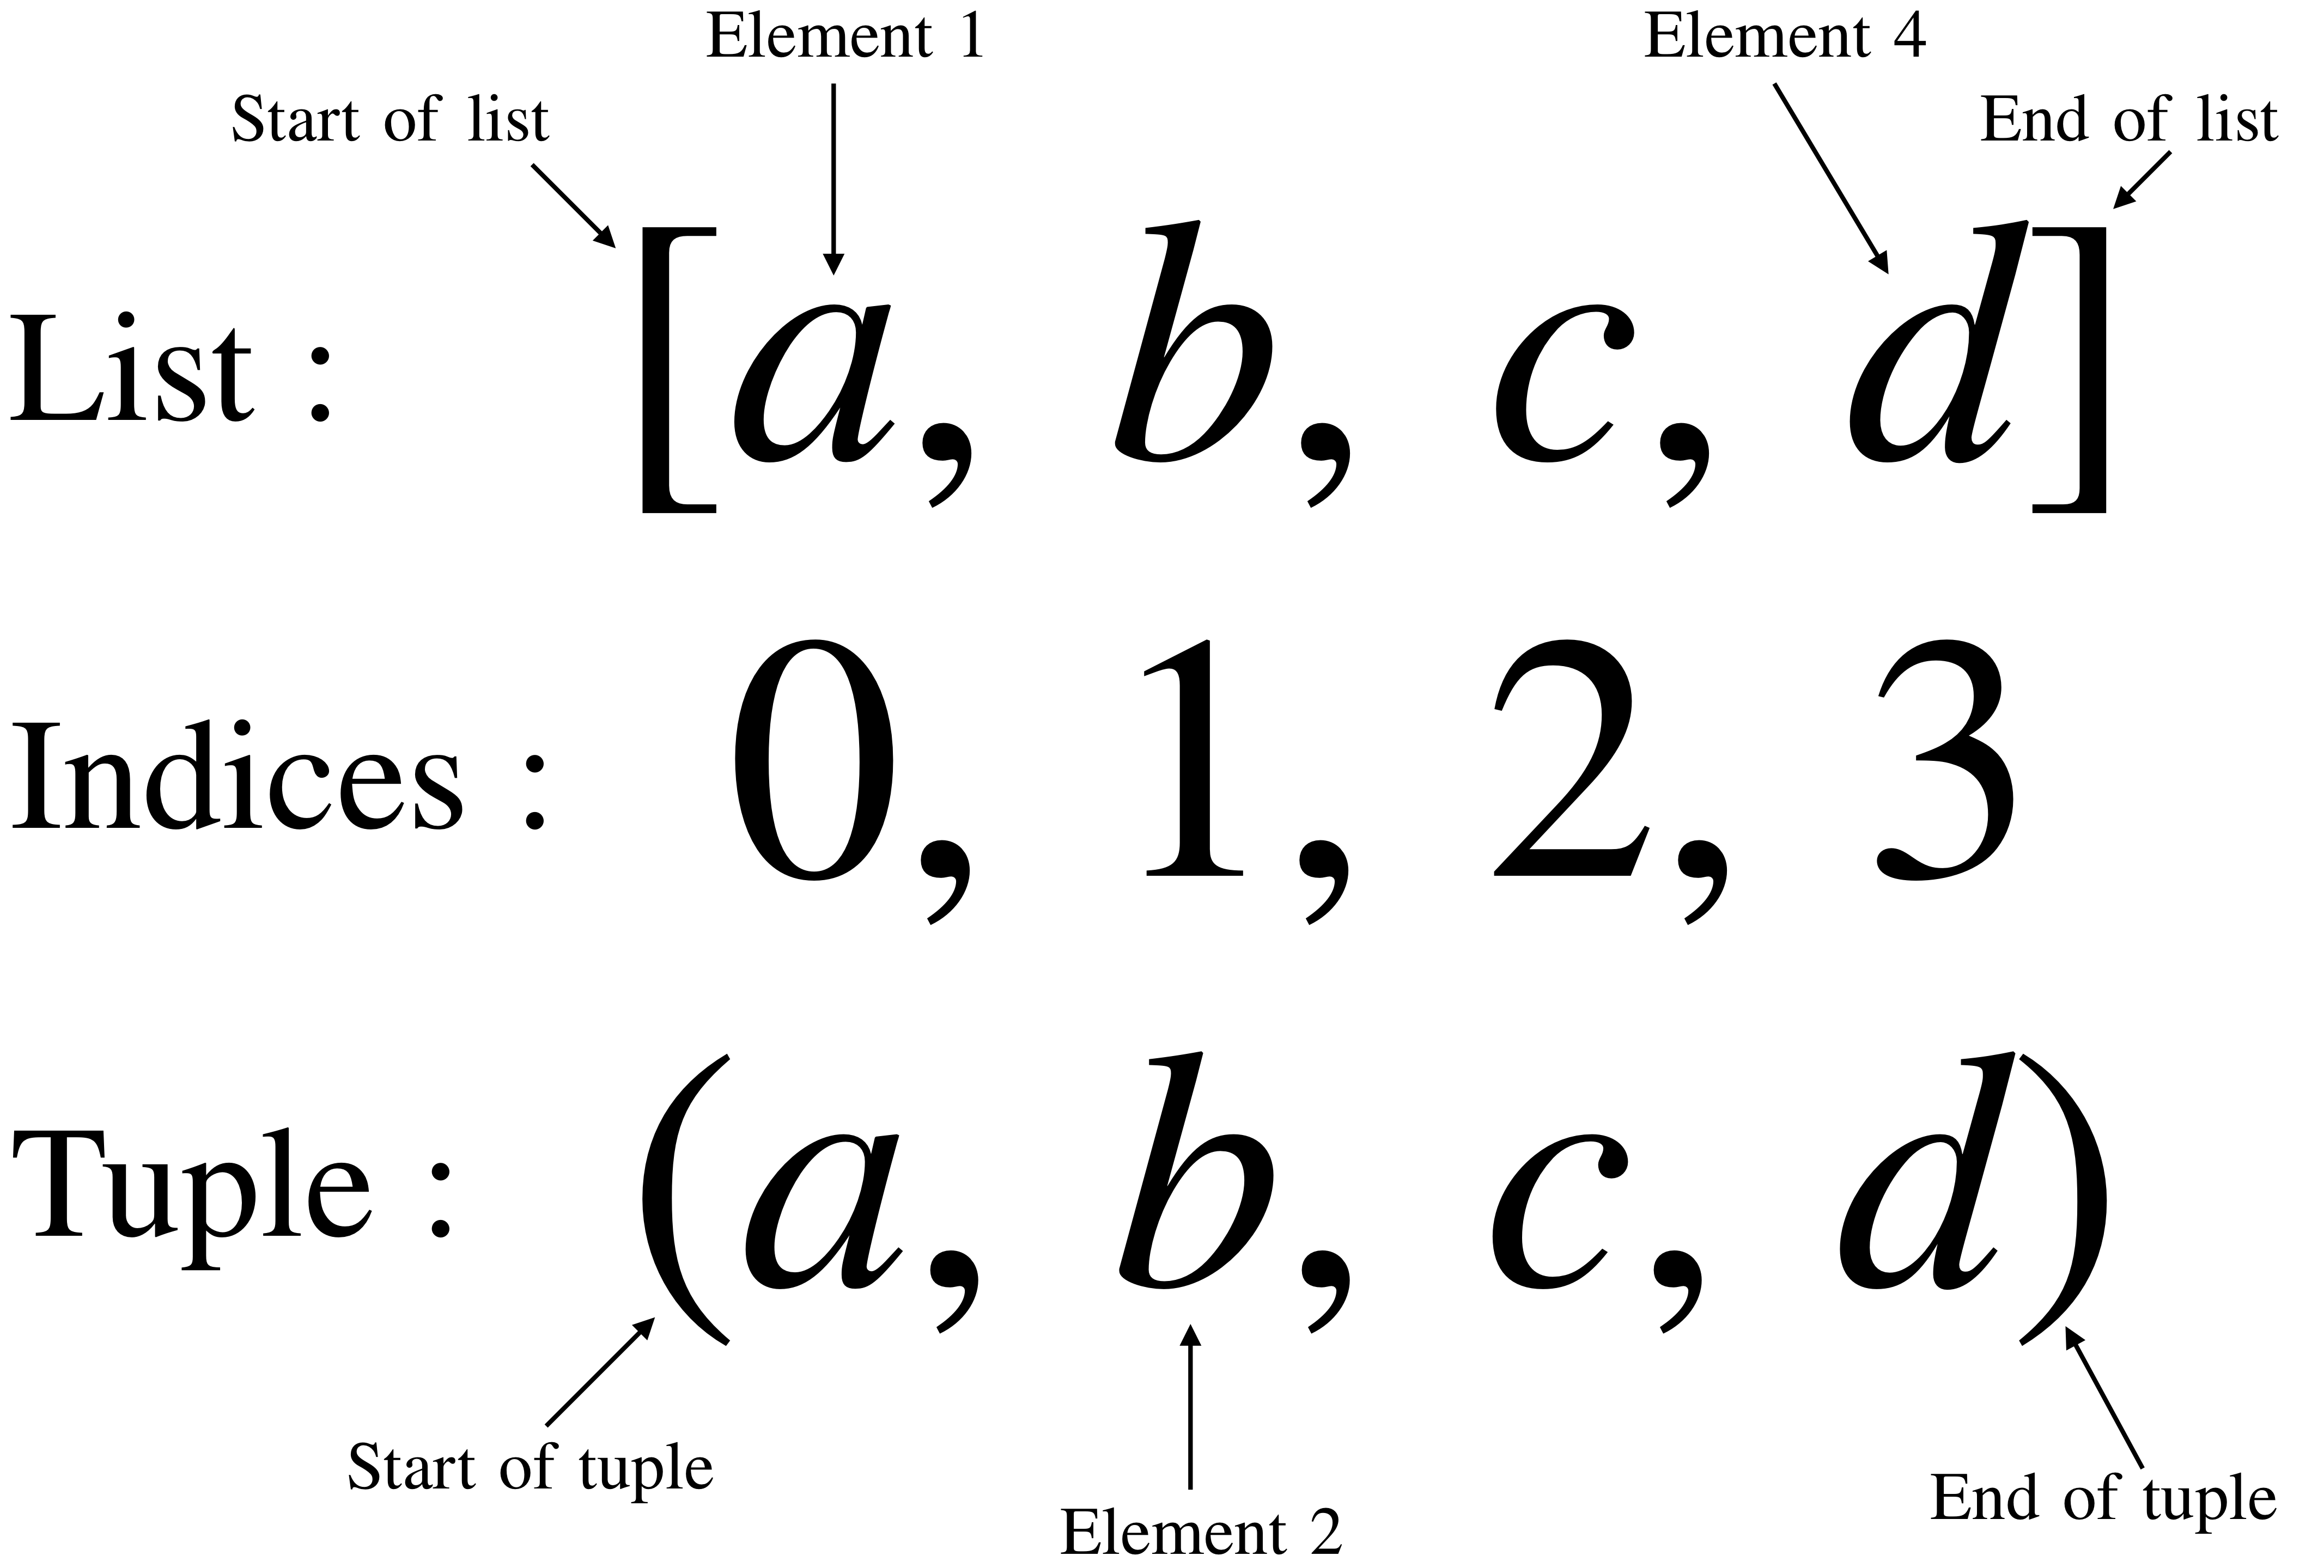
\includegraphics[width=0.6\linewidth]{Figures/ListTup.png}
\caption{A diagram showing the anatomy of \texttt{python} tuples and lists. Lists, tuples and strings all have the same index conventions where the first element is the zeroth element. The way a list is differentiated from a tuple is the symbol used to denote the beginning and end of each; for a list \texttt{[]} and for a tuple \texttt{()}.} 
\label{fig:listtup}
\end{figure}

\subsection{Tuples}
\label{sec:Tuples}
\noindent Once a tuple has been declared, it cannot be changed or edited in any way. A tuple is declared using parentheses `\texttt{( )}' to surround the elements (the contents of the list), which must be separated by commas. You can also create a tuple containing only one element, by putting a comma after the first entry in the tuple (i.e. \texttt{(element1,)}). 

\begin{lstlisting}[style=PY] 
In [1]: # Define a simple 1 element tuple
        simpletuple = (5, )
        
        print(simpletuple)
\end{lstlisting}
\begin{lstlisting}[style=PY_out]
        (5, )
\end{lstlisting}
\begin{lstlisting}[style=PY]
In [2]: # Redefine the simple tuple contain multiple elements
        simpletuple = (5, 4, 3, 2, 1)
        
        print(simpletuple)
\end{lstlisting}
\begin{lstlisting}[style=PY_out]
        (5, 4, 3, 2, 1)
\end{lstlisting}
We can index a tuple just as we have indexed strings to extract individual elements.
\begin{lstlisting}[style=PY]
In [3]: # Extract and print the third element in the tuple
        print(simpletuple[2])
\end{lstlisting}
\begin{lstlisting}[style=PY_out]
        3
\end{lstlisting}
Rather than indexing every time we want a specific element from a tuple we can also extract each element into its own variable, effectively naming that element of the tuple. Notice here the LHS has the right number of variables to extract each element into its own individual variable; if this is not the case an error well be raised telling you there were ``Too many values to unpack".\\

\noindent What happens if you leave out the quotation marks around \textit{Bruce}, and do you remember why?
\begin{lstlisting}[style=PY] 
In [4]: # Define a new tuple of strings
        name = ('Bruce', 'Batman', 'Wayne')
        print(name)
        
        # `Name' (assign to a variable) each element of the tuple
        firstname, superHeroName, lastname = name
        print(firstname)
\end{lstlisting}
\begin{lstlisting}[style=PY_out]
        ('Bruce', 'Batman', 'Wayne')
        Bruce
\end{lstlisting}
We can then use the variables containing individual elements.
\begin{lstlisting}[style=PY]
In [5]: print("*Gruff Voice* I am " + superHeroName)
\end{lstlisting}
\begin{lstlisting}[style=PY_out]
        *Gruff Voice* I am Batman
\end{lstlisting}
As with a string, we can slice the tuple to extract a range of elements, here the first and second. Lists can be sliced in exactly the same way.
\begin{lstlisting}[style=PY]
In [6]: # Extract the first and second element of the tuple and print
        print(name[0:2])
\end{lstlisting}
\begin{lstlisting}[style=PY_out]
        ('Bruce', 'Batman')
\end{lstlisting}
We can also combine all of these together along with some string slicing (remember what adding strings together is called and put it in a comment) .
\begin{lstlisting}[style=PY]
In [7]: print("*Gruff Voice* I am " + name[0] + " " + lastname[0:2] 
               + "... I mean " + superHeroName)
\end{lstlisting}
\begin{lstlisting}[style=PY_out]
        *Gruff Voice* I am Bruce Wa... I mean Batman
\end{lstlisting}

\newpage

\subsection{Lists}
\label{sec:lists}
\noindent Lists, unlike tuples, are mutable and can be edited; this feature means they tend to be used a lot more than tuples. Lists are defined by using square brackets `\texttt{[ ]}' with elements separated by commas (just as in a tuple).\\

\noindent Useful list methods (functions used by putting a dot after a variable) include:
\begin{itemize}
    \item \texttt{append} - adds an element to the end of a list.
    \item \texttt{extend} - add a list of elements to the end of a list.
    \item \texttt{insert} - which allows you to add an element at a given position.
    \item \texttt{pop} - this removes and returns an element at a given position.
\end{itemize}

\noindent Another very useful function is \texttt{len}, which will return the number of elements in a list (this also works with strings, so \texttt{len("python")} would return \textbf{6}. Just like strings and tuples, lists can be indexed and sliced to extract certain elements.

\begin{lstlisting}[style=PY] 
In [1]: # Define a list
         alist = [2, 4, 6]
        
         # Append 10 to the end of the list 
         # (add an element to the end) 
         alist.append(10) 
        
         print(alist)
\end{lstlisting}
\begin{lstlisting}[style=PY_out]
        [2, 4, 6, 10]
\end{lstlisting}
\begin{lstlisting}[style=PY]
In [2]: len(alist)  # Get the length of the list
\end{lstlisting}
\begin{lstlisting}[style=PY_out]
Out[2]: 4
\end{lstlisting}

Here is an example of the use of the insert method compared to simply overwriting elements in the list.

\begin{lstlisting}[style=PY]
In [3]: # Insert 8 into the 4th position (index 3) within the list
        alist.insert(3, 8)
         
        print(alist)
\end{lstlisting}
\begin{lstlisting}[style=PY_out]
        [2, 4, 6, 8, 10]
\end{lstlisting}
\begin{lstlisting}[style=PY]
In [4]: # Overwrite elements 3 and 4 (index 2 and 3) with strings
        alist[2:4] = ['Something', 'to']
        
        print(alist)
\end{lstlisting}
\begin{lstlisting}[style=PY_out]
        [2, 4, 'Something', 'to', 10]
\end{lstlisting}

\begin{table}[H]
\begin{center}
\begin{tabular}{|l | p{6.5cm}|}
\hline
\multicolumn{2}{|c|}{\textbf{For use with strings, tuples, and lists:}} \\\hline
\texttt{a + b} & Joins items together\\\hline
\texttt{a[i:j]} & Outputs elements from \textit{i} to \textit{j}-1 of a \\\hline
\texttt{a[i]} & Outputs \textit{i}$^{th}$ element of a\\\hline
\texttt{x * a} & Produces x copies of a\\\hline
\texttt{len(a)} & Outputs length of a \\\hline
\multicolumn{2}{|c|}{\textbf{For use with a tuple or a list only:}} \\\hline
\texttt{min(a)} & Outputs minimum value in a\\\hline
\texttt{max(a)} & Outputs maximum value in a\\\hline
\texttt{n in a} & Outputs true if element n is in a\\\hline
\multicolumn{2}{|c|}{\textbf{For use with lists only:}} \\\hline
\texttt{a.append(x)} & Adds element x to list a at the end\\\hline
\texttt{a.insert(n,x)} & Adds element x to list a in position n\\\hline
\texttt{a.extend(x\_list)} & Adds the elements in \texttt{x\_list} to list a at the end\\\hline
\texttt{a.pop(x\_list)} & Removes and returns an element at a given position\\\hline
\end{tabular}
\end{center}
\caption {Operators for strings, tuples and lists}
\label{StringTab}
\end{table}

\begin{tcolorbox}[colback=red!5!white,colframe=red!75!black]
\subsection{The \texttt{is} Keyword}
As well as checking if variables are equal you can check if two variables are literally the same object with the \texttt{is} keyword. This can be useful when programs get complex and copies of lists get involved (more on this later). 

With variables defined as integers, floats, or strings \texttt{is} behaves the same as \texttt{==}, which was introduced in section \ref{boolvars} (also where the \texttt{a} and \texttt{c} variables were defined).
\begin{lstlisting}[style=PY]
In [1]: # Define a new variable d which IS a
        d = a
        e = 12
        
        # Test if c is d
        print(c is d)
        
        # Test if a is d
        print(a is d)
        
        # Test if d is e and a is e
        print(d is e and a is e)
\end{lstlisting}
\begin{lstlisting}[style=PY_out]
        False
        True
        True
\end{lstlisting}
Here it is obvious that \texttt{d} is \texttt{a} and \texttt{c} is not \texttt{d}. The important thing to note is that when using lists (or any \texttt{Python} variable more complex than a integer, float, or string) \texttt{is} will return \texttt{False} even when two variables contain the same elements. This is because the two variables are different instances of the \texttt{Python} object and are located at different memory addresses.

\begin{lstlisting}[style=PY]
In [2]: # Define new variables containing the same list
        list1 = [1, 2, 3]
        list2 = [1, 2, 3]
        list3 = list1  # Making an alias!
        
        # Test if list1 equals list2 and if it equals list3
        print(list1==list2, list1==list3)
        
        # Test if list1 is list2 and if it is list3
        print(list1 is list2, list1 is list3)
\end{lstlisting}
\begin{lstlisting}[style=PY_out]
        True True
        False True
\end{lstlisting}
If you \textbf{assign a list to a new variable} (this is called aliasing - like the example above) and edit the new variable you will be \textbf{editing the original}! To avoid this you can test using \texttt{`is'}. The same rules also stand for tuples, though remember they are immutable and can't be edited.
\end{tcolorbox}
\begin{tcolorbox}[colback=red!5!white,colframe=red!75!black]
 Essentially the linked copy is just another name (an alias) for the original variable. To make an independent copy you can use the slice operator (but omit the start and end indices to take the whole list) or you can use the \texttt{copy} method.
\begin{lstlisting}[style=PY]
In [3]: # Define a list
        lst = ['Aliasing', 'causes', 'me', 'so', 'many', 'problems']
        
        # Create an alias for the list
        alias_lst = lst
        
        # Create a copy with each method
        lst_copy1 = lst[:]
        lst_copy2 = lst.copy()
        
        # Test if the list is equal to the alias and copies
        print(lst==alias_lst, lst==lst_copy1, lst==lst_copy2)
        
        # Test if the list is the alias and copies
        print(lst is alias_lst, lst is lst_copy1, lst is lst_copy2)
\end{lstlisting}
\begin{lstlisting}[style=PY_out]
        True True True
        True False False
\end{lstlisting}
\end{tcolorbox}

\subsection{Exercises}

\begin{enumerate}
\item W2Basic3 - Create a tuple variable `top5' with 5 elements containing your favourite animals.
\begin{enumerate}
      \item Check if `dog' is in your tuple, such that it displays {\tt true} or {\tt false} (see Tab. \ref{StringTab}).
      \item Print the 3$^{\text{rd}}$ item in your tuple.\\
\end{enumerate}

\item W2Basic4 - Create a list called `mylist' containing 10 numbers.
\begin{enumerate}
      \item Print the length of the list.
      \item Print the minimum value in the list.
      \item Print the maximum value in the list.
      \item Add the number 14 to your list of numbers and print the new length.
      \item Insert (using the insert function) the number 8 to the 9$^{th}$ place in the list.
      \item Print the elements 5 through 9 (i.e. 5 numbers) in your list. Note the last element printed should be 8.
\end{enumerate}
\end{enumerate}

\section{Input function}
The \texttt{input} function is used to get a response from the user of a program, this will be your first interactive use of \texttt{Python}! An example can be seen below:
\begin{lstlisting}[style=PY] 
In [1]: # Get the users name and assign it to a variable
        name = input('Name: ')
        
        print('Hello ' + name)
\end{lstlisting}
\begin{lstlisting}[style=PY_out] 
        Name: |...
\end{lstlisting}
The input function will print the provided string and then output will hang waiting for user input. If the user then writes Batman for instance, the rest of the code following the input statement will be executed having assigned the Batman to the \texttt{name} variable.
\begin{lstlisting}[style=PY_out] 
        Name: Batman
        Hello Batman
\end{lstlisting}

The \texttt{input} function will always return a string, so don't let this catch you out. If you need an integer input from the user you have to convert the string returned by \texttt{input} to an integer, like so:
\begin{lstlisting}[style=PY] 
In [2]: # Get a number from the user, convert to an integer
        print('Choose a number')
        num = int(input('Number: '))
        
        # Multiply this number by 5 and print the result
        print('5 times your number is:')
        print(5 * num)
\end{lstlisting}
which for the input of 5 results in
\begin{lstlisting}[style=PY_out] 
        Choose a number
        Number: 5
        5 times your number is:
        25
\end{lstlisting} 
This takes your number and multiplies it by 5.

%% \subsection{Input in \texttt{Python} 2.7}
%% As we have said, we use \texttt{Python} 3 in this sub-module, but you may come across \texttt{Python} 2.7 at some point in your degree and/or career. In \texttt{Python} 2.7, you would use {\tt raw\_input} rather than {\tt input}.

%% \vspace{0.25cm}
%% \begin{tcolorbox}[colback=red!5!white,colframe=red!75!black]
%% Python 2.7 is "dead" as of January 1st 2020 (no longer supported, think of 2.7 like an old car where you can't buy the parts to fix it anymore) - any Googling you do, try to be careful of which version of \texttt{Python} the post or guide is using.
%% \end{tcolorbox}

\subsection{Issues with \texttt{jupyter}}
Sometimes with the \texttt{input} function (though occasionally with others), you might see a \texttt{jupyter} cell that looks like this:
\begin{lstlisting}[style=PY] 
    In  [*]:
\end{lstlisting}

\noindent and you are unable to get any outputs from any of the cells in your notebook. If this happens, essentially \texttt{jupyter} has frozen. Simply click on the "Kernel" dropdown menu and restart the notebook, and bear in mind that restart and clear all will remove all of your \texttt{Out} cells. Any form of restart will remove all previously defined variables from memory, meaning you'll have to run all your code again.
\subsection{Exercises}

\begin{enumerate}
\item W2Basic5 - Calculate a tip for a meal
    \begin{enumerate}
      \item Create a short set of commands (in one \texttt{jupyter} cell), that allows the user to enter the price of their meal in a restaurant.
      \item Then print out a message displaying a price including a 15\% and 20\% tip.
    \end{enumerate}

\item W2Basic6 - Calculating your age in seconds
    \begin{enumerate}
      \item Create a short set of commands (in one \texttt{jupyter} cell), that allows the user to enter their age at their last birthday. Assign this value to a variable \texttt{age}.
      \item Use the \texttt{age} variable to calculate their approximate age in seconds (ignore leap years).
      \item Print `You are over N seconds old', where N is their age in seconds..
    \end{enumerate}
\end{enumerate}

\section {Signpost} 

You should have at least reached this point by the end of the lab session in week 2. If you are here with plenty of time to spare, then you have several options:

\begin{enumerate}
    \item Leave now (though get an AT to check that you've done enough first).
    \item Start on the first assessment/competency test.
    \item Work through some of the advanced problems in section \ref{firstadvanced} (\textbf{this is the preferred option}).
\end{enumerate}

\newpage
\section{Advanced Exercises - Some independent learning may be required}
\label{firstadvanced}

\begin{enumerate}
\item Print out hello world so it looks like the this using only one print command:
\begin{lstlisting}[style=PY_out] 
Out [1]: Hello
         World!
\end{lstlisting}
\noindent Hint: Think invisible characters...

\item Given the diameter of the sun is 1,391,000 km, print out the time in years (as an integer) it would take to drive round the sun's circumference at 100 kilometres per hour. (Take $\pi$ as 3.141)
\item Create a string variable called \texttt{animal} and assign an animal to it. Using one print command print \texttt{animal} on five different lines.
\item Create a list called colours, containing two elements `red' and `green'.
\begin{enumerate}
\item Add `blue' and `yellow' to the list, put it in alphabetical order, and print it.
\item Remove `yellow' from the list.
\item Print the list in reverse.
\item Make an independent copy of `colours' called `RGB'
\item Add `yellow' back to colours.
\item Print `{\tt colours=}' and `{\tt RGB=}', note: {\tt colours} should contain one more entry than {\tt RGB}.
\item Show (using a Boolean) that `colours' and `RGB' are not equal in length.
\end{enumerate}
\item Create a tuple called `Words' containing 5 words of your choice and print the item.
\begin{enumerate}
\item Using the slice operator, slice words such that the second and third words are printed.
\item Find an alternate slicing method to produce the same result as above.
\end{enumerate}
\end{enumerate}

\newpage

\section{Worked Solutions for Section \ref{Strings}}
\label{workedanswerslab2}

\begin{lstlisting}[style=PY] 
In [1]: # Worked solution for Week 1, Exercise 1a
        # Define two string variables
        first_word = "Hello"
        second_word = "World"
        
        # Concatenating, with a space, and assigning to new variable
        full_sentence = first_word + " " + second_word
        
        # Printing the finished phrase
        print(full_sentence)
\end{lstlisting}

\begin{lstlisting}[style=PY_out] 
        Hello World
\end{lstlisting}

\begin{lstlisting}[style=PY] 
In [2]: # Worked solution for Week 1, Exercise 1b
        # Printing out the string 20 times
        print(first_word*20)
\end{lstlisting}
\begin{lstlisting}[style=PY_out] 
        hellohellohellohellohellohellohellohellohellohellohellohellohellohello
        hellohellohellohellohellohello
\end{lstlisting}

\begin{lstlisting}[style=PY] 
In [3]: # Worked solution for Week 1, Exercise 2a
        # Define the string variable
        warning_phrase = "Do not push the red button"
        
        # Printing the warning phrase, because I can
        print(warning_phrase)
\end{lstlisting}
\begin{lstlisting}[style=PY_out] 
        Do not push the red button
\end{lstlisting}

\begin{lstlisting}[style=PY] 
In [4]: # Worked solution for Week 1, Exercise 2b
        # Slicing and printing in one line
        print(warning_phrase[:11])
\end{lstlisting}
\begin{lstlisting}[style=PY_out] 
        Do not push
\end{lstlisting}

\begin{lstlisting}[style=PY] 
In [5]: # Worked solution for Week 1, Exercise 2c
        # Slicing differentently for another phrase
        print(warning_phrase[7:])
\end{lstlisting}
\begin{lstlisting}[style=PY_out] 
        push the button
\end{lstlisting}
